		\begin{objectives}
			In this tutorial you will explore some modelling with both ODEs and PDEs and you will study the stability of equilibrium solutions.
			
				These problems relate to the following course learning objectives:
				\begin{itemize}\it 
					\item Model with ODEs. \\[-20pt]
					\item Analyze equilibria and their stability. \\[-20pt]
					\item Model with PDEs.
				\end{itemize}
		\end{objectives}



\vspace{-.5em}
\subsection*{Problems}
\vspace{-.5em}


\begin{enumerate}


	\item \label{q1}\footnote{Based on the 2020 test 2.} 
	The von Bertalanffy-P\"utter type tumour growth model is
	\[
	\frac{dv}{dt} = pv^a - qv^b \quad , \quad v(0) = v_0,
	\]
	in which $v(t)$ is the volume of the tumour in mm$^3$ at time $t$ in days. 
	The parameters are $p > 0$, $q > 0$, and $b > a > 0$. 
	The first term $pv^a$ corresponds to resources (nutrients, oxygen, energy, etc) entering the tumour, while the second term $-qv^b$ corresponds to resource consumption by the tumour.
	
	\begin{enumerate}
		\item \label{q1:stabilities} What are the two equilibrium tumour volumes? What are their stabilities?
		\item Explain why this model predicts that the tumour volume grows monotonically.
		
		\textit{Hint: Use the results from part (\ref{q1:stabilities}) to help you.}
		
		\item What is the sensitivity of the (non-trivial) equilibrium tumour volume with respect to $p$? How does this sensitivity depend on the nominal value of $p$ and $q$?
		
		\item If we assume that resources are consumed proportionally to the number of cells, what is the value of $b$? Call this value $b_0$.

		\item If we assume that the resources enter the tumour through its surface area and that the tumour is approximately spherical, what is the value of $a$? Call this value $a_0$.

		\item The volume of a breast tumour was measured from medical images. The data is shown below in circles. The curve is the least squares best-fit of the model using $a = a_0$ and $b = b_0$, which gives $p = 0.72$ and $q = 0.036$. 
		What ultimate tumour size does this predict? How trustworthy is this prediction?

		
		\begin{center}
			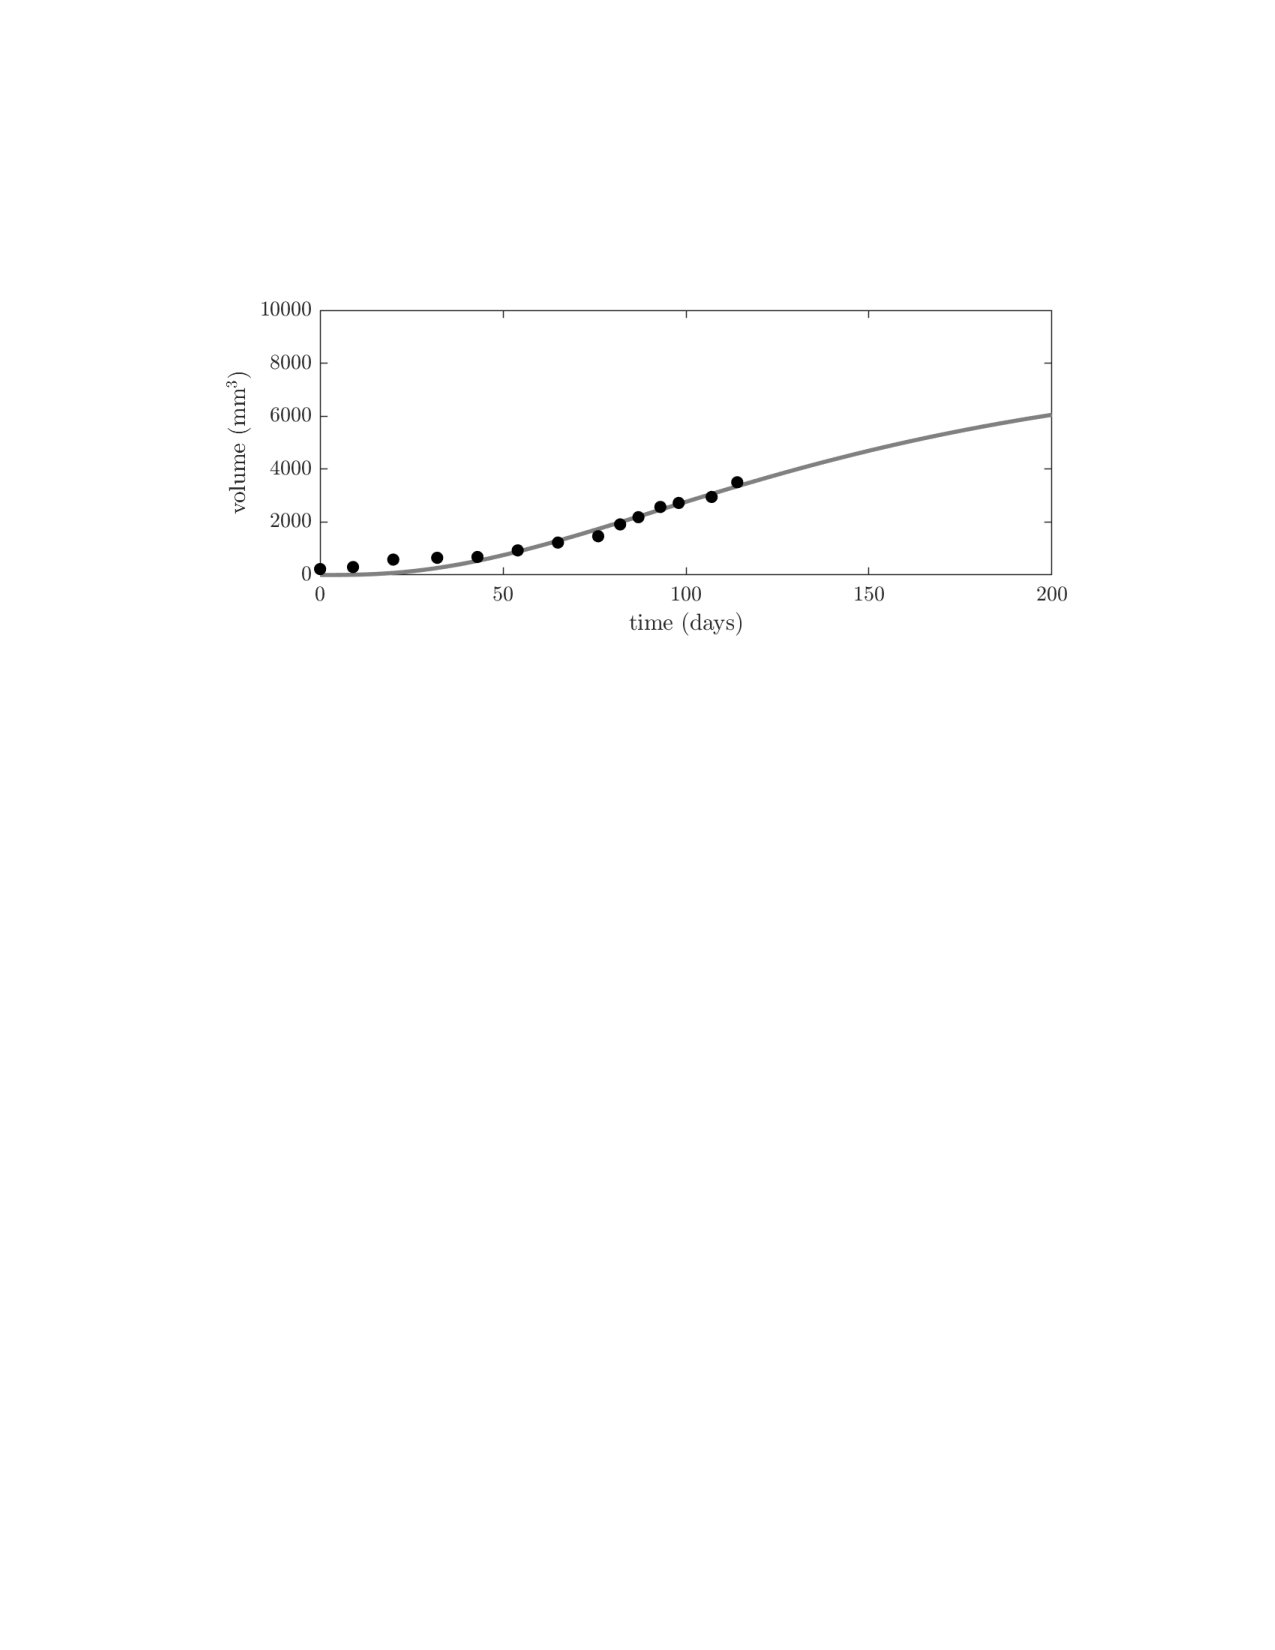
\includegraphics[width=.65\textwidth]{tumour.pdf}
		\end{center}
		
		
			
	\end{enumerate}

	\newpage

	\item\label{q2}\footnote{Based on the 2024 test 2.} 
	A particular highway has two lanes in the same direction. The density of vehicles in lane $i = 1, 2$ is $\rho_i(x, t)$ at position $x$ down the highway and time $t$. 
	The continuum traffic model with the Greenshields velocity model is
	\begin{align*}
		\frac{\partial \rho_1}{\partial t} + \frac{\partial}{\partial x} \left[ \rho_1 v_{\max}(1-\rho_1/\rho_{\max})\right] & = 	\alpha (\rho_2 - \rho_1) \\[10pt]
		\frac{\partial \rho_2}{\partial t} + \frac{\partial}{\partial x} \left[ \rho_2 v_{\max}(1-\rho_2/\rho_{\max})\right] & = 	\alpha (\rho_1 - \rho_2)
	\end{align*}

	
	\begin{enumerate}
		\item \label{ex:Q} What does 
		\[
		Q = \int_{-\infty}^{\infty} \rho_1 + \rho_2 ~dx
		\] 
		represent? Assume that the flux goes to 0 as $x$ approaches $\pm \infty$ and show that $Q$ is constant in time.
		
		
		\item What do the terms $\alpha (\rho_2-\rho_1)$ and $\alpha(\rho_1 - \rho_2)$ represent? Discuss the reasonableness of these terms as a model for what they represent.
		
		
		\item How would you change this model to account for the fact that $n(t)>0$ cars get into the highway at the position $x=2$. What do you expect to happen to the quantity $Q$ from part (\ref{ex:Q})?
		
	\end{enumerate}

	
		
	
\end{enumerate}
















